\section{Exact polynomial certificates}\label{sec:certificates}

This appendix proves the finite polynomial inequalities used in
Section~\ref{sec:coupling}. The coefficients are rational throughout.
The certificates are those of \cite[Section~7]{OpenAI2026P}.
We give the conversion formulas, domains, and coefficient bounds so
that each sign follows from a finite polynomial expansion.
The method uses the nonnegative Bernstein basis on intervals and
simplices; see Boudaoud--Caruso--Roy~\cite{BoudaoudCarusoRoy2008} and
Roy~\cite[Sections~1 and~4]{Roy2007}. We prove the conversion formulas
and their matrix-valued consequence here. Positivity is verified for
these specific polynomials, with their boundary zeros retained.
The accompanying source package contains a standard-library Python
checker at \path{verification/}. From the source package's root,
the exact coefficient calculations can be reproduced with
\begin{verbatim}
python -B verification/verify.py --check
\end{verbatim}

\subsection{Bernstein coefficients on intervals and triangles}

\begin{lemma}[Bernstein conversion]\label{lem:bernstein-conversion}
Let $p$ be a polynomial of degree at most $N$ on an interval $[r,s]$,
and write
\[
 p(r+(s-r)z)=\sum_{j=0}^N a_jz^j.
\]
Its degree-$N$ Bernstein expansion is
\[
 p(r+(s-r)z)=\sum_{i=0}^N h_i\binom Ni z^i(1-z)^{N-i},
 \qquad
 h_i=\sum_{j=0}^i a_j\frac{\binom ij}{\binom Nj}.
\]
In particular, $h_i\ge\eta$ for all $i$ implies $p\ge\eta$ on
$[r,s]$.

For a polynomial on a triangle with ordered vertices
$p_\ell=(r_\ell,s_\ell)$, set
\[
 V=r_3+(r_1-r_3)z+(r_2-r_3)w,\qquad
 W=s_3+(s_1-s_3)z+(s_2-s_3)w.
\]
If $P(z,w)=p(V,W)=\sum_{d,e}P_{de}z^dw^e$ has degree at most $N$,
then its normalized degree-$N$ triangular coefficients are
\[
 [p]_{ij}=s_{ij}(P):=
 \sum_{d=0}^i\sum_{e=0}^j
 \frac{\binom id\binom je}
      {\binom N{d+e}\binom{d+e}d}\,P_{de},
 \qquad i,j\ge0,\quad i+j\le N.
\]
On $z,w\ge0$, $z+w\le1$, the polynomial is the sum of these coefficients
times the nonnegative basis functions
\[
 \frac{N!}{i!j!(N-i-j)!}
       z^iw^j(1-z-w)^{N-i-j}.
\]
These basis functions sum to one. The same expansion applies entrywise
to a symmetric polynomial matrix: positive semidefiniteness of every
coefficient matrix implies positive semidefiniteness throughout the
triangle.
\end{lemma}

\begin{proof}
For an interval, expand
$z^j=z^j(z+(1-z))^{N-j}$ and compare coefficients in the Bernstein
basis. On a triangle, expand
\[
 z^dw^e=z^dw^e(z+w+(1-z-w))^{N-d-e}.
\]
This gives the displayed factors after dividing each coefficient by the
corresponding multinomial coefficient. Equivalently, substitute
\[
 (v,b)=\frac{u_1p_1+u_2p_2+u_3p_3}{u_1+u_2+u_3}
\]
and multiply by $(u_1+u_2+u_3)^N$. The normalized coefficient of
$u_1^iu_2^ju_3^{N-i-j}$ is $[p]_{ij}$. The positivity statements
follow from the nonnegative partition of unity, also for matrix
quadratic forms.
\end{proof}

\subsection{The quartic scalar certificates}

\begin{lemma}[Scalar certificates]\label{lem:scalar-certificates}
For the polynomials in Section~\ref{sec:coupling}, the following bounds
hold:
\[
\begin{gathered}
 C_0>0,\qquad
 4C_0\left((h-A_0)(2-v)+\frac25hv\right)
       -(2-v)(2A_0+L_0)^2>0\quad(0\le v\le2),\\
 G,H>0\quad(0\le u\le1),\qquad
 Z_*\le0\quad(0\le u\le1/16),\\
 Z_*^2\le64A^2u^2GH\quad(1/16\le u\le1).
\end{gathered}
\]
\end{lemma}

\begin{proof}
Apply the interval formula of Lemma~\ref{lem:bernstein-conversion} in
the degrees and on the intervals indicated below. Every coefficient
has at least the displayed positive lower bound. In the first two rows
the bound applies on each of the two intervals separately.
\begin{center}
\small
\begin{tabular}{@{}lccc@{}}
\toprule
Polynomial & Degree & Interval & Lower bound\\
\midrule
$C_0$ & $2$ & $[0,1],\ [1,2]$ & $1/2$\\
$4C_0((h-A_0)(2-v)+\frac25hv)
 -(2-v)(2A_0+L_0)^2$
 & $5$ & $[0,1],\ [1,2]$ & $1/2$\\
$G$ & $4$ & $[0,1]$ & $9/10$\\
$H$ & $4$ & $[0,1]$ & $1/4$\\
$-Z_*$ & $8$ & $[0,1/16]$ & $13/100$\\
$64A^2u^2GH-Z_*^2$ & $16$ & $[1/16,1]$ & $12/100$\\
\bottomrule
\end{tabular}
\end{center}
For the first two rows the coefficients are in fact strictly greater
than $1/2$. For example, their respective minima on the two intervals are
\[
 \left(\frac{3971}{3200},\frac{1063}{1600}\right),
 \qquad
 \left(\frac{101027}{20000},\frac{283729}{400000}\right).
\]
All entries in this table are obtained by substituting the displayed
formulas for $A_0,L_0,C_0$ and for $A,G,H,L,Z_*$ into the coefficient sum in
Lemma~\ref{lem:bernstein-conversion}. Thus each bound is an inequality
between rational coefficients. The lemma proves the required signs.
\end{proof}

\subsection{The two matrix certificates}

For the quadratic inequality \eqref{eq:22}, introduce
\[
\begin{aligned}
 r_v&=1+6v+v^2,\qquad r_b=1+6b+b^2,
       \qquad \alpha=\frac54,\\
 H_v&=8vK\Theta(1+v)
       -r_v\left\{vD+K\left[v(X_v+\partial_v\kappa)
                                      +\frac{2\kappa}{3}\right]\right\},\\
 H_b&=H_v(b,v),\\
 S_*&=4(\alpha+\alpha^{-1})vb
       +\frac{\alpha b(1-v)^2+\alpha^{-1}v(1-b)^2}{2}.
\end{aligned}
\]
The diagonal differences in \eqref{eq:22} are
$H_v/(vKr_v)$ and $H_b/(bKr_b)$. Since
$r_v=8v+(1-v)^2$ and $r_b=8b+(1-b)^2$, weighted arithmetic--geometric
mean gives
\[
 \sqrt{vb r_vr_b}
       \le\frac{\alpha b r_v+\alpha^{-1}v r_b}{2}=S_*.
\]
It is therefore sufficient to prove
\[
 \begin{pmatrix}H_v&S_*KJ\\S_*KJ&H_b\end{pmatrix}\succeq0.
\]
Indeed its diagonal entries are nonnegative and its determinant gives
$H_vH_b\ge S_*^2K^2J^2\ge vb r_vr_bK^2J^2$. Dividing by the positive
denominators proves that the matrix of differences in \eqref{eq:22}
is positive semidefinite. This argument uses $J^2$ and imposes no sign
condition on $J$.

For a symmetric $2\times2$ matrix, record its entries in the order
$(11,22,12)$ as a triple $(r,h',s')$. In this notation the two triples
to be certified are
\[
\begin{aligned}
 \mathcal A={}&P_0\bigl(v(K_1,K_2,K_{12})-\kappa(5,1,0)\bigr)
       -2v^2(P_k^2,P_l^2,P_kP_l),\qquad \sigma=1,\\
 \mathcal B={}&(H_v,H_b,S_*KJ).
\end{aligned}
\]
The first triple is precisely the matrix in \eqref{eq:21} at
$\sigma=1$.

\begin{lemma}[Matrix and boundary certificates]
\label{lem:matrix-certificates}
The symmetric matrix represented by $\mathcal A$ is positive semidefinite on
\[
 \mathcal D=\{(v,b):v,b\ge0,\ v+b\le2\}.
\]
The symmetric matrix represented by $\mathcal B$ is positive semidefinite on
\[
 \mathcal D_+=\{(v,b)\in\mathcal D:v\ge b\}.
\]
On $\mathcal D_+$ one also has
\[
 L_v\ge0,\qquad F+12c\delta^2L_b\ge0.
\]
\end{lemma}

\begin{proof}
Use the vertices
\[
\begin{gathered}
 O=(0,0),\quad S=(1,0),\quad C=(1,1),\quad
 U=(2,0),\quad W_0=(0,2),\\
 A=(1/2,1/2),\quad B=(3/2,1/2),\quad E=(1,1/2).
\end{gathered}
\]
A three-letter word specifies the vertices of an ordered triangle.
The triangles $OSC$, $OCW_0$, and $SCU$ cover $\mathcal D$.
The triangles $OAS$, $ASE$, $ACE$, $SBE$, $CBE$, and $SUB$ cover
$\mathcal D_+$; the latter is also the single triangle $OCU$, or the
union $OSC\cup SCU$. All edges are included. The two subdivisions are
shown in Figure~\ref{fig:certificate-domains}.

\begin{figure}[htbp]
\centering
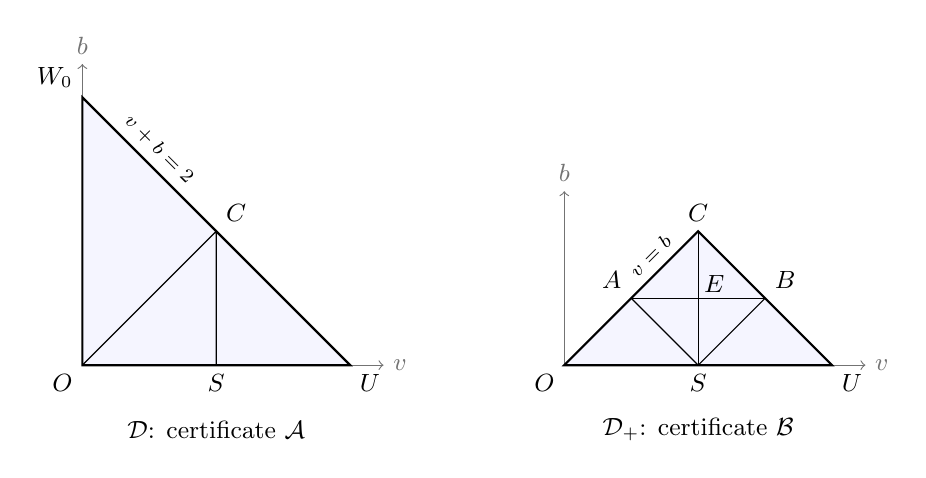
\begin{tikzpicture}[scale=1.7, every node/.style={font=\small}]
 \begin{scope}
  \fill[blue!4] (0,0)--(2,0)--(0,2)--cycle;
  \draw[->,black!55] (0,0)--(2.25,0) node[right] {$v$};
  \draw[->,black!55] (0,0)--(0,2.25) node[above] {$b$};
  \draw[thick] (0,0)--(2,0)--(0,2)--cycle;
  \path (2,0)--(0,2) node[pos=.76,above,sloped,font=\scriptsize]
    {$v+b=2$};
  \draw (0,0)--(1,1)--(1,0);
  \node[below left] at (0,0) {$O$};
  \node[below] at (1,0) {$S$};
  \node[below right] at (2,0) {$U$};
  \node[above right] at (1,1) {$C$};
  \node[above left] at (0,2) {$W_0$};
  \node at (1,-0.48) {$\mathcal D$: certificate $\mathcal A$};
 \end{scope}
 \begin{scope}[xshift=3.6cm]
  \fill[blue!4] (0,0)--(2,0)--(1,1)--cycle;
  \draw[->,black!55] (0,0)--(2.25,0) node[right] {$v$};
  \draw[->,black!55] (0,0)--(0,1.3) node[above] {$b$};
  \draw[thick] (0,0)--(2,0)--(1,1)--cycle;
  \path (0,0)--(1,1) node[pos=.73,above,sloped,font=\scriptsize]
    {$v=b$};
  \draw (0.5,0.5)--(1,0)--(1.5,0.5);
  \draw (1,0)--(1,1);
  \draw (0.5,0.5)--(1.5,0.5);
  \node[below left] at (0,0) {$O$};
  \node[below] at (1,0) {$S$};
  \node[below right] at (2,0) {$U$};
  \node[above] at (1,1) {$C$};
  \node[above left] at (0.5,0.5) {$A$};
  \node[above right] at (1.5,0.5) {$B$};
  \node[above right,inner sep=2pt] at (1,0.5) {$E$};
  \node at (1,-0.48) {$\mathcal D_+$: certificate $\mathcal B$};
 \end{scope}
\end{tikzpicture}
\caption{Subdivisions of the Weyl-norm domains
$\mathcal D=\{(v,b):v,b\ge0,\ v+b\le2\}$ and
$\mathcal D_+=\mathcal D\cap\{v\ge b\}$ used in the triangular
coefficient table. Every edge is included. The norm condition
$v+b\le2$ is a necessary relaxation of the sectional-curvature condition;
the tensor estimates retain the stronger constraint $x+y\le2$.}
\label{fig:certificate-domains}
\end{figure}


For a matrix row, the last two columns below bound, respectively,
\[
 \min([r]_{ij},[h']_{ij}),\qquad
 [r]_{ij}[h']_{ij}-[s']_{ij}^{2}.
\]
Thus the last column is the determinant of each coefficient matrix.
For a scalar row, the first bound applies directly to its coefficient.
The bounds apply to every nonzero coefficient; a zero matrix exception
means that all three of its entries vanish.
\begin{center}
\small
\begin{tabular}{@{}lcccrr@{}}
\toprule
Object & Triangle & $N$ & Zeros &
 \shortstack{Diagonal or\\scalar bound} & Determinant bound\\
\midrule
$\mathcal A$ & $OSC$ & $8$ & $0$ & $16000$ & $53000000$\\
 & $OCW_0$ & $8$ & $0$ & $890$ & $3900000$\\
 & $SCU$ & $8$ & $0$ & $2400$ & $3500000$\\
\midrule
$\mathcal B$ & $OAS$ & $9$ & $0$ & $43$ & $1050$\\
 & $ASE$ & $9$ & $0$ & $43$ & $490$\\
 & $ACE$ & $10$ & $1$ & $2$ & $21$\\
 & $SBE$ & $9$ & $0$ & $43$ & $1300$\\
 & $CBE$ & $10$ & $2$ & $13/100$ & $4$\\
 & $SUB$ & $9$ & $0$ & $5$ & $290$\\
\midrule
$L_v$ & $OCU$ & $6$ & $1$ & $9/10$ & ---\\
$F+12c\delta^2L_b$ & $OSC$ & $9$ & $6$ & $19/100$ & ---\\
 & $SCU$ & $9$ & $7$ & $9/1000$ & ---\\
\bottomrule
\end{tabular}
\end{center}

Here are explicit expansion instructions for all entries of the table.
They also fix the coefficient ordering. Write
$a=V-1$, $s=W-1$ in \eqref{eq:15} and form $\kappa(V,W)$ and
its two partial derivatives. A partial derivative is obtained by
reducing the appropriate exponent of each monomial and multiplying by
that exponent. Differentiate before substituting the affine expressions
$V,W$. Put
\[
 \kappa_* =\kappa(V,W),\qquad \bar\kappa_* =\kappa(W,V).
\]
Thus the partial derivatives of the exchanged function, before affine
substitution, are
\[
 \partial_V\bar\kappa_*(V,W)=(\partial_2\kappa)(W,V),\qquad
 \partial_W\bar\kappa_*(V,W)=(\partial_1\kappa)(W,V).
\]

Ordinary coefficient arrays are multiplied by convolution:
\[
 (PQ)_{de}=\sum_{f=0}^d\sum_{g=0}^e P_{fg}Q_{d-f,e-g}.
\]
Use
\[
\begin{aligned}
 m_*&=\left(1-\frac38(V-W)\right)^2,
       &d_0&=2-V-W,\\
 P_{k,*}&=300m_*+160h d_0,
       &P_{l,*}&=35m_*V,\\
 Y_*&=m_*(42+3W^2+10V^2)
       -h\bigl[6(V^2+W^2-V-W)-26d_0\bigr].
\end{aligned}
\]
For $\mathcal A$, apply $s_{ij}$ from
Lemma~\ref{lem:bernstein-conversion} to the three entries of
\[
\begin{aligned}
 &(P_{k,*}+30hV)
       \bigl\{V(A_1,Y_*,A_{12})-\kappa_*(5,1,0)\bigr\}\\
 &\hspace{22mm}-2V^2(P_{k,*}^2,P_{l,*}^2,P_{k,*}P_{l,*}),
\end{aligned}
\]
where
\[
 A_1=5Y_*+m_*(300V+140V^2)+160h d_0V,
 \qquad
 A_{12}=m_*(75V+35V^2)+40h d_0V.
\]
These are the original entries of \eqref{eq:21} at $\sigma=1$, expressed
only in the affine polynomials $V,W$.

For $\mathcal B$, put
\[
\begin{aligned}
 K_*&=4+V^2+W^2,\qquad \Theta_* =\Theta(V,W),\\
 X_*&=m_*(-70+100V-25V^2-5W^2)
       +\frac53h\bigl(6(a^2+s^2)+32a d_0\bigr),\\
 H_*&=8VK_*\Theta_*(1+V)\\
 &\quad-(1+6V+V^2)
       \left\{VD+K_*\left[V\bigl(X_*+(\partial_1\kappa)(V,W)\bigr)
                                     +\frac{2\kappa_*}{3}\right]\right\}.
\end{aligned}
\]
Apply $s_{ij}$ to $H_*$, to its exchange in $V,W$, and to
\[
 S_*(V,W)\left\{
       \frac{K_*}{2}\bigl((\partial_2\kappa)(V,W)
                        +(\partial_2\kappa)(W,V)\bigr)-D\right\}.
\]
For example, on $CBE$ the triples at $(i,j)=(8,0),(8,1),(8,2)$ are
\[
 \left(\frac{11041}{810},\frac{4063}{810},\frac{60557}{16200}\right),
 \quad
 \left(\frac{4328}{405},\frac{839}{405},\frac{3977}{2700}\right),
 \quad
 \left(\frac{191}{81},\frac{191}{81},-\frac{1189}{1350}\right).
\]

For the two scalar rows, apply $s_{ij}$ to
$10h d_0V-\kappa_*$ and, respectively, to
\[
\begin{aligned}
 c(V,W)\bigg\{&D\left(1-\frac{d_0^2}{4}\right)(V-W)^2
       +30h d_0(V^2a^2+W^2s^2)\\
 &+6(Va\kappa_*+Ws\bar\kappa_*)
       +12d_0^2(10h d_0W-\bar\kappa_*)\bigg\}-\Theta_*^2.
\end{aligned}
\]
Together with the coefficient-sum formula, these prescriptions produce
the displayed rational bounds by addition and multiplication of finite
arrays.

The zero exceptions are as follows, with the third homogeneous index
always $N-i-j$. For $\mathcal B$, they are the vertex $C$ in $ACE$
and $CBE$, namely $(0,10,0)$ and $(10,0,0)$, and also $(9,1,0)$ in
$CBE$. For $L_v$ the only zero is $(0,6,0)$, the vertex $C$ in $OCU$.
For $F+12c\delta^2L_b$ on $OSC$, the zeros are exactly $i+j\le2$.
On $SCU$ they are exactly $9-j\le2$, together with $(i,j)=(0,6)$.
There are no other exceptions.

Every nonzero matrix coefficient has positive diagonal entries and
positive determinant, and each exceptional matrix is zero. Thus all
coefficient matrices are positive semidefinite. The scalar coefficients
are all nonnegative. Lemma~\ref{lem:bernstein-conversion} and the stated
domain coverage prove the assertions.
\end{proof}

\subsection{The remaining potential polynomial}

\begin{lemma}[The polynomial $F$]\label{lem:potential-certificate}
The polynomial $F=cE_0-\Theta^2$ is nonnegative on $\mathcal D$.
\end{lemma}

\begin{proof}
Use $v=1-n+t$, $b=1-n-t$. The full domain becomes
\[
 0\le n\le1,\qquad |t|\le1-n.
\]
Write $F_*(n,t)=F(1-n+t,1-n-t)$ for the pullback to these coordinates.
It is even in $t$, and direct expansion gives
$F_*=\sum_{j=0}^4 f_j(n)t^{2j}$, where
\[
\begin{aligned}
 240f_0={}&n^3(1-n)\bigl(53511n^4-151593n^3
                 +222537n^2-83607n+10256\bigr),\\
 60f_1={}&n\bigl(19389n^5-418926n^4+523719n^3
                 -289776n^2+67782n+10564\bigr),\\
 60f_2={}&-1260129n^4+1370598n^3-451164n^2+23442n+74,\\
 10f_3={}&-12200n^2+2601n+75,\qquad
 f_4=-\frac{23}{5}.
\end{aligned}
\]
For $n<1$, put $z=t^2/(1-n)^2\in[0,1]$. The degree-four Bernstein
coefficients in $z$ are
\[
 h_i(n)=\sum_{j=0}^i
       \frac{\binom ij}{\binom4j}f_j(n)(1-n)^{2j},
 \qquad 0\le i\le4.
\]
Define
\[
 d_0(n)=n^3(1-n),\qquad d_1(n)=n(1-n),\qquad
 d_2(n)=d_3(n)=d_4(n)=1-n.
\]
Each quotient $q_i=h_i/d_i$ is a polynomial. Applying the interval
conversion formula to it on each of the four intervals
\[
 [0,1/4],\quad[1/4,1/2],\quad[1/2,3/4],\quad[3/4,1]
\]
gives the following lower bounds for every coefficient:
\begin{center}
\begin{tabular}{@{}cccc@{}}
\toprule
$i$ & Divisor $d_i$ & Degree of $q_i$ & Lower bound\\
\midrule
$0$ & $n^3(1-n)$ & $4$ & $3$\\
$1$ & $n(1-n)$ & $6$ & $31$\\
$2$ & $1-n$ & $7$ & $1/5$\\
$3$ & $1-n$ & $7$ & $12/5$\\
$4$ & $1-n$ & $7$ & $9/5$\\
\bottomrule
\end{tabular}
\end{center}
The complete prescription for each entry is to insert the displayed
$f_j$ into $h_i$, cancel the indicated polynomial factor, and apply
the coefficient sum in Lemma~\ref{lem:bernstein-conversion} in the
listed degree. In particular, the identities $h_i=d_iq_i$ hold as
polynomial identities, including at the endpoints.

Since every $d_i$ is nonnegative on $[0,1]$, every $h_i$ is
nonnegative. Therefore
\[
 F_*=\sum_{i=0}^4h_i(n)\binom4i z^i(1-z)^{4-i}\ge0
 \qquad(n<1).
\]
At $n=0$, the coordinate $z=t^2$ still covers the entire permitted
interval $|t|\le1$; the vanishing of $h_0,h_1$ causes no difficulty.
At $n=1$, the domain contains only $t=0$, and directly
$F_*(1,0)=F(0,0)=f_0(1)=0$. Thus no numerical division by a vanishing factor
is required, and all of $\mathcal D$ is covered.
\end{proof}

Lemmas~\ref{lem:scalar-certificates}, \ref{lem:matrix-certificates},
and \ref{lem:potential-certificate} establish every polynomial
inequality used in Section~\ref{sec:coupling}. Hence the three estimates
of Proposition~\ref{prop:coupling-estimates} hold on the stated
positive-variable spectral domain. The compatible limit in
Section~\ref{sec:coupling} extends them to the zero sets under the
nonnegative sectional-curvature hypothesis.
